\section{Preliminaries}
\subsection{Notation}
The set of integers and real numbers are denoted $\int$ and $\real$ respectively. A ranged subset of a space is denoted with $\mathbb{S}\rii{i}{j}=\{s\in\mathbb{S}|i\leq s\leq j\}$. Parenthesis are used in place of brackets to denote strict inequalities. Open bounds are defined using notation such as $\mathbb{S}\rgeq{i}$ where any comparison operator can be substituted for $\geq$. Define the set of integers from $1$ to $k>1$ as $\idxset{k}\triangleq\int\rii{1}{k}$.\edit{ Use $\PowerSet{\cdot}$ to denote the power set of a finite set.}{}

A directed graph \edit{}{with $\gnumnodes\in\int\rgeq{1}$ nodes} is defined as $\graph\triangleq\{(\gnodeedges{n},\gnodelabel{n})\}_{n\in\idxset{\gnumnodes}}$ where \edit{$\gnodeedges{n}\in\PowerSet{\idxset{\gnumnodes}}$}{$\gnodeedges{n}\subseteq\idxset{\gnumnodes}$} lists the successor nodes of node $n$ and \edit{$\gnodelabel{n}=\idxset{\gnumlabels}$ is the node's label}{$\gnodelabel{n}\in\idxset{\gnumlabels}$ is an integer label assigned to node $n$ where $\gnumlabels$ is the max integer label}. A discrete, time varying function, \edit{$f(t)$ mapping to a graph's nodes}{$f:\int\rgeq{0}\rightarrow\idxset{\gnumnodes}$}, is said to respect the graph if $f(t)=n$ implies that $f(t+1)\in\gnodeedges{n}$. The set of all such functions for a specific graph, $\graph$ is denoted $\Sigma(\mathcal{G})\triangleq\{g:\int\rgeq{0}\rightarrow\idxset{\gnumnodes}\ |\ g(\cdot)\text{ respects }\graph\}$. 
\begin{remark}
Note that a function $f(\cdot)\in\Sigma(\graph)$ maps to a node, not the node's label. The active label at time $t$ can be accessed with $\gnodelabel{f(t)}$. 
\end{remark}

\subsection{Switching Signals}
An external switching signal is any discrete function, \edit{$\ss(\cdot)$}{$\ss:\int\rgeq{0}\rightarrow \idxset{\gnumnodes}$,} that is uninfluenced by the system's state and control inputs and causes elements of the plant and/or controller to switch. In this work, the switching signals are constrained using directed graphs \edit{. A directed graph is defined as $\graph\triangleq\{(\gnodeedges{n},\gnodelabel{n})\}_{n\in\idxset{\gnumnodes}}$ where $\gnodeedges{n}\in\PowerSet{\idxset{\gnumnodes}}$ lists the successor nodes of node $n$ and $\gnodelabel{n}=\idxset{\gnumlabels}$ is the node's label. A switching signal that maps to a graph's nodes is said to respect the graph if $\sigma(t)=n$ implies that $\sigma(t+1)\in\gnodeedges{n}$. The set of all such signals for a specific graph, $\graph$ is denoted $\Sigma(\mathcal{G})\triangleq\{\sigma:\int\rgeq{0}\rightarrow\idxset{\gnumnodes}\ |\ \sigma(\cdot)\text{ respects }\graph\}$.}{such that, given the graph $\graph$, $\ss(\cdot)\in\Sigma(\graph)$.} At time $t$, the active node's label indicates the system's mode and is defined as $\ssl(t)\triangleq \gnodelabel{\ss(t)}$. Using directed graphs to constrain the switching signal generalizes dwell time and successor constraints from previous literature such as \cite{Danielson2019, Hall2022, Zhang2016}, representing a richer set of constraints, as shown in \autoref{fig:graph_ex}.

\begin{figure}[t]
\centering
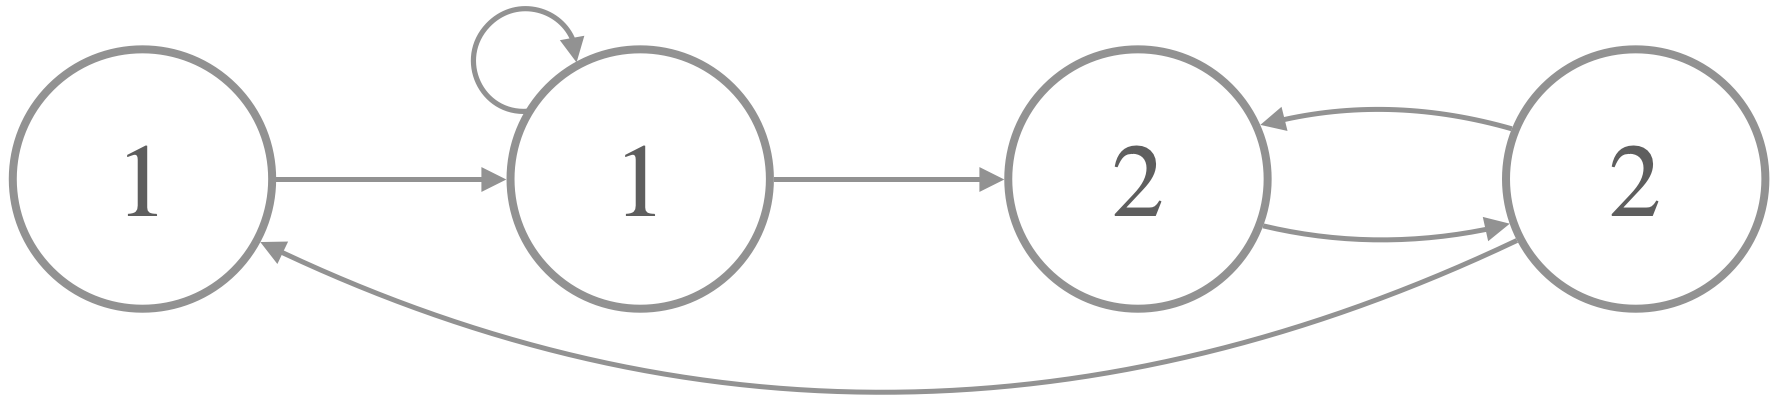
\includegraphics[scale=0.15]{./figures/graph_remark}
\caption{\edit{A graph representing a 2-mode system where the first mode has a minimum dwell time of 2 while the second mode can only be left during odd dwell times.}{A graph representing a 2-mode system. The system is in mode 1 when node 1 or 2 is active and in mode 2 otherwise. Note that, when the system switches to mode 1 by entering node 1, it must ``dwell'' in mode 1 for at least 2 steps. This is equivalent to a minimum dwell time constraint found in works such as \cite{Danielson2019}.}}
\label{fig:graph_ex}
\end{figure}

Prior knowledge of the switching signal is not required, but its value at time $t$ is known immediately. Furthermore, its directed graph is known at design time. 
\subsection{General Constrained Switched Systems}
Switched systems \edit{}{in the context of this work} are comprised of \edit{}{\nummodes} modes and \edit{}{a graph based} switching constraint\edit{s}{ $\graph$ where the labels of the graph correspond to the system's mode indices, $\nummodes=\gnumlabels$}. Each mode contains the dynamics and constraints that the system must respect while the mode is active. A single mode is denoted using the tuple
\begin{equation}
\mode{\modeidx}\triangleq\{f_\modeidx\in \mathcal{D}^{\nx,\nu,\nw}, \xcon[\modeidx]\subseteq\real^\nx, \ucon[\modeidx]\subseteq\real^\nu, \wcon[\modeidx]\subset\real^\nw\}\nonumber
\end{equation}
where $\mathcal{D}^{\nx,\nu,\nw}\triangleq\{f:\real^{\nx\times\nu\times\nw}\rightarrow\real^\nx\}$ defines the set of discrete dynamics,  and $\xcon[\modeidx]$, $\ucon[\modeidx]$, and  $\wcon[\modeidx]$ are the state, input, and disturbance constraints respectively. The full constrained switched system collects the modes and a directed graph \edit{to take the form}{into}
\begin{equation}\label{eq:basic_switched_sys}
\modes\triangleq\{\{\mode{\modeidx}\}_{\modeidx\in\idxset{\nummodes}}, \graph\}.
\end{equation}
\edit{where the labels of the graph correspond to a mode index, $\gnumlabels=\nummodes$.}{}

\subsection{Set Operations and Control Invariance}
Set operations provide tools to analyze how a mode evolves under allowable inputs. Given a mode, $\mode{\modeidx}$, the following important set operation is introduced. 
%\begin{definition}[Robust Preset]\label{def:robust_preset}
%The $k$-step, robust preset of a set $\mathcal{S}$ under the constrained dynamics $\mode{\modeidx}$ is given by
%\begin{align}
%\Pre[\modeidx][0]{\mathcal{S}}&\triangleq\mathcal{S},\\
%\Pre[\modeidx][k]{\mathcal{S}}&\triangleq\{x\in\xcon[\modeidx]\ |\ \exists u\in\ucon[\modeidx]\text{ s.t. }\forall w\in\wcon[\modeidx],\nonumber\\ &\qquad f_\modeidx(x,u,w)\in\Pre[\modeidx][k-1]{\mathcal{S}}\}.
%\end{align}
%\end{definition}
\begin{definition}[Previewed Robust Preset]\label{def:prev_robust_preset}
The $k$-step, previewed robust preset of a set $\mathcal{S}$ under the constrained dynamics $\mode{\modeidx}$ is given by
\begin{align}
\PreviewedPre[\modeidx][0]{\mathcal{S}}&\triangleq\mathcal{S},\\
\PreviewedPre[\modeidx][k]{\mathcal{S}}&\triangleq\{x\in\xcon[\modeidx]|\forall w\in\wcon[\modeidx],\exists u\in\ucon[\modeidx]\text{ s.t. }\nonumber\\
&\hspace{1.85cm} f_\modeidx(x,u,w)\in\PreviewedPre[\modeidx][k-1]{\mathcal{S}}\}.
\end{align}
\end{definition}
Comparing this to the more common robust preset operator, the previewed robust preset is allowed to select the input based on a known disturbance. The previewed robust preset is used when the system is allowed a preview of the current disturbance. This preview can expand the size of the preset because the selected input need not handle every possible disturbance. 

For linear systems where $f_\modeidx(x,u,w) = A_\modeidx x + B_\modeidx u + E_\modeidx w$, previewed robust presets can be found using basic set operations such as the Minkowski sum and difference as shown below and adapted from \cite{Borrelli2017}.
\begin{align*}
\PreviewedPre[\modeidx][1]{\mathcal{S}} &= \left(\left(\left(\mathcal{S}\oplus\left(-B_\modeidx\circ\ucon[\modeidx]\right)\right)\ominus E_\modeidx\circ\wcon[\modeidx]\right)\circ A_\modeidx\right)\ \cap\ \xcon[\modeidx].
\end{align*}

Preset operations are critical in the calculation of invariant sets commonly used in feasibility analysis. \edit{An invariant set is}{Control invariant and previewed-robust control invariant sets are} defined as follows.
\begin{definition}[\Ac{ci} sets \cite{Dorea1999}]\label{def:ci_set}
A set, $\mathcal{S}\subseteq\xcon[\modeidx]$ is CI under mode $\mode{\modeidx}$ if for all $x\in\mathcal{S}$, there exists a $u\in\ucon[\modeidx]$ such that \edit{$f_\modeidx(x,u,w)\in\mathcal{S}$.}{$f_\modeidx(x,u,0)\in\mathcal{S}$. Likewise, a set $\mathcal{S}\subseteq\xcon[\modeidx]$ is a previewed robust CI (PR-CI) set if, for all $x\in\mathcal{S}$ and $w\in\mathcal{W}_\modeidx$, there exists a $u\in\ucon[\modeidx]$ such that $f_\modeidx(x,u,w)\in\mathcal{S}$.} Equivalently, $\mathcal{S}$ is CI\edit{}{ (PR-CI)} iff $\mathcal{S}\subseteq\Pre[\modeidx][1]{\mathcal{S}}$\edit{.}{ where the preset operator is nominal (previewed robust).}
\end{definition}
\edit{ This definition holds regardless of if the preset operator is nominal, robust, or previewed robust.}{}

A final tool used in this paper is the convex hull of a set defined as follows.
\begin{definition}[Convex Hull]
Given a set $\mathcal{S}\subseteq\real^n$, the convex hull is defined as 
\begin{align*}
&\Call{ConHull}{\mathcal{S}}\triangleq\\&\{x\in\real^n\ |\ \exists\ a,b\in\mathcal{S},\ \gamma\in\real\rii{0}{1}\ \text{s.t.}\ x=\gamma a + (1-\gamma)b\}.
\end{align*}
\end{definition}
\subsection{Feasibility Analysis}
\edit{In constrained systems, it is extremely important that the controller can satisfy the state constraints using only feasible inputs. If a feasible input exists that results in a feasible state, the system is feasible. If feasibility at the current time implies feasibility at all future times, then the system is persistently feasible.}{}

\edit{In centralized, unswitched systems, persistent feasibility can be established by constraining the system to be within a \ac{ci} set, $\mathcal{C}\subseteq\mathcal{X}$ \cite{Blanchini1999}. Relying on constant, control invariant sets becomes difficult in externally switched systems, however. The \ac{ci} set must be common to all system modes or else persistent feasibility is lost. This concern can be addressed using time varying, control invariant sets that take advantage of constraints on the switching signal. For example, in \cite{Danielson2019,Santis2004,Lavaei2021,Athanasopoulos2017}, time varying, control invariant sets were developed that force the system to move during the dwell time between switches to a region from which a switch to any successor mode will preserve persistent feasibility. By bounding the dwell time below, the system had additional time to reach these safe regions, thereby loosening the state constraints.}{}

\edit{The approaches used in the previous literature can be described using safe-set collections.}{The introduction, it was mentioned that by constraining the external switching signal allows a time-invariant feasible region to be replaced with a time-varying one. This work describes these time-varying feasible regions using safe-set collections} These are collections of sets, indexed by the switching signal, that serve as time-varying state constraints of the system. To establish persistent feasibility, every safe-set must be within the 1-step preset of all possible successor safe-sets. This is presented formally in the following definition.
\begin{definition}[Safe-set collection]
Let the external switching signal, $\ss\in\Sigma(\graph)$ govern the system $\modes\triangleq\{\{\mode{\modeidx}\}_{\modeidx\in\idxset{\nummodes}}, \graph\}$. A collection of sets indexed by the nodes of $\graph$, $\mathcal{S}=\{\mathcal{S}_{i}\}_{i\in\idxset{\gnumnodes}}$ is a safe-set collection if
$$\mathcal{S}_{i}\subseteq\Pre[\gnodelabel{j}][1]{\mathcal{S}_{j}}\ \forall\ i\in\idxset{\gnumnodes},\ j\in \gnodeedges{i}$$
\end{definition}
Safe set collections create target sets for the system to move into at each time step. The preset condition ensures that, no matter how $\ss$ evolves, \edit{the system will always be able to find a}{there will always be a} feasible input \edit{to move into the current target set}{that moves the state into the current target set}.
